% Created 2017-10-23 Mon 23:36
% Intended LaTeX compiler: pdflatex
\documentclass[11pt,xcolor=dvipsnames]{beamer}
\usepackage[utf8]{inputenc}
\usepackage[T1]{fontenc}
\usepackage{graphicx}
\usepackage{grffile}
\usepackage{longtable}
\usepackage{wrapfig}
\usepackage{rotating}
\usepackage[normalem]{ulem}
\usepackage{amsmath}
\usepackage{textcomp}
\usepackage{amssymb}
\usepackage{capt-of}
\usepackage{hyperref}
\newcommand{\bottomcite}[1]{\fbox{\vbox{\footnotesize #1}}}
\usepackage{multicol}
\usepackage[utf8]{inputenc}
\usepackage[T1]{fontenc}
\usepackage[portuguese]{babel}
\usepackage{textcomp}
\usepackage{graphics}
\usepackage{tikz}
\usepackage{listings}
\usepackage{lmodern}
\graphicspath{{../img/}{./img/}}
\newcommand{\copyleft}{\includegraphics[width=0.5cm]{cc_cc_30.pdf}\hspace{0.2cm}\includegraphics[width=0.5cm]{cc_by_30.pdf}\hspace{0.2cm}\includegraphics[width=0.5cm]{cc_sa_30.pdf}}
\newcommand{\infufrgs}{\includegraphics[width=1cm]{inf-ufrgs-bw.pdf}}
\usepackage{tabularx}
%\setbeamercolor{title}{fg=black}
%\setbeamercolor{titlelike}{fg=black}
%\setbeamercolor{itemize item}{fg=black}
%\setbeamercolor{itemize subitem}{fg=black}
%\setbeamercolor{itemize subsubitem}{fg=black}
\setbeamertemplate{footline}[frame number]
\setbeamertemplate{navigation symbols}{}
\setbeamersize{text margin left=.5cm}
\setbeamersize{text margin right=.5cm}
\newcommand{\murl}[2]{{#1://#2}}
\newcommand{\et}[1]{{\scriptsize\texttt{#1}}}
\newcommand{\etn}[1]{{\texttt{#1}}}



\usetheme{default}
\author{schnorr}
\date{\today}
\title{Reproducibility \linebreak (CMP595 PPGC/INF/UFRGS)}
\hypersetup{
 pdfauthor={schnorr},
 pdftitle={Motivation for a Rigourous Analysis \linebreak (CMP595 PPGC/INF/UFRGS)},
 pdfkeywords={},
 pdfsubject={},
 pdfcreator={Emacs 25.2.2 (Org mode 9.0.1)}, 
 pdflang={English}}
\begin{document}

{\setbeamertemplate{footline}{} 

\author{Lucas Mello Schnorr, Jean-Marc Vincent}

\date{INF/UFRGS \newline Porto Alegre, Brazil -- October 20th, 2017}

\titlegraphic{
    
\includegraphics[scale=1.4]{./logo/ufrgs2.png}
    \hspace{1cm}
    
\includegraphics[scale=1]{./logo/licia-small.png}
    \hspace{1cm}
    
\includegraphics[scale=0.3]{./logo/uga.png}
}
\maketitle
}

\label{sec-1}
\begin{frame}[label=sec-1-0-1]{Frustration as an Author }
\begin{itemize}
\item I thought I used the same parameters but \alert{I'm getting different
results!}
\item The new student wants to compare with \alert{the method I proposed last
year}
\item My advisor asked me whether I took care of setting this or this but
I can't remember
\item The damned fourth reviewer asked for a major revision and wants me
to \alert{change figure 3} :(
\item \alert{Which code} and \alert{which data set} did I use to generate this figure?
\item It \alert{worked yesterday}!
\item 6 months later: \alert{why} did I do that?
\end{itemize}
\end{frame}
\begin{frame}[label=sec-1-0-2]{Frustration as a Reviewer }
This may be an interesting contribution but:
\begin{itemize}
\item This \alert{average value} must hide something
\item As usual, there is no \alert{confidence interval}, I wonder about the
variability and whether the difference is \alert{significant} or not
\item That can't be true, I'm sure they \alert{removed some points}
\item Why is this graph in \alert{logscale}? How would it look like otherwise?
\item The authors decided to show only a \alert{subset of the data}. I wonder
what the rest looks like
\item There is no label/legend/\ldots{} What is the \alert{meaning of this graph}?
If only I could access the generation script
\end{itemize}
\end{frame}
\begin{frame}[label=sec-1-0-3]{A Few Edifying Examples }
\begin{columns}
  \begin{column}{.67\linewidth}
    \bottomcite{Naicken, Stephen \textit{et Al.}, \textit{Towards Yet
        Another Peer-to-Peer Simulator}, HET-NETs'06.}\medskip\\
    \small
    From 141 P2P sim.papers, 30\% use a custom tool, \alert{50\% don't report
    used tool}\\ \medskip

  \end{column}
  \begin{column}{.33\linewidth}
    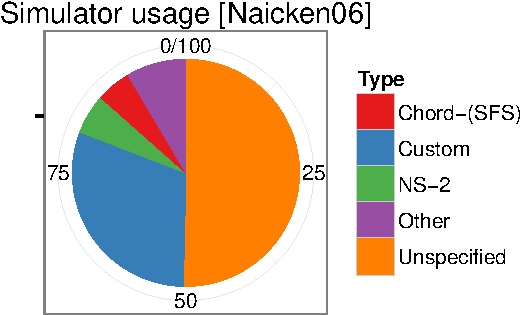
\includegraphics[width=\linewidth]{img/naicken.pdf}
  \end{column}
\end{columns}

\bottomcite{Collberg, Christian \textit{et Al.}, \textit{Measuring
    Reproducibility in Computer Systems Research},
  \url{http://reproducibility.cs.arizona.edu/}}

\begin{columns}
  \begin{column}{.5\linewidth}
    ~\hspace{-1.7em}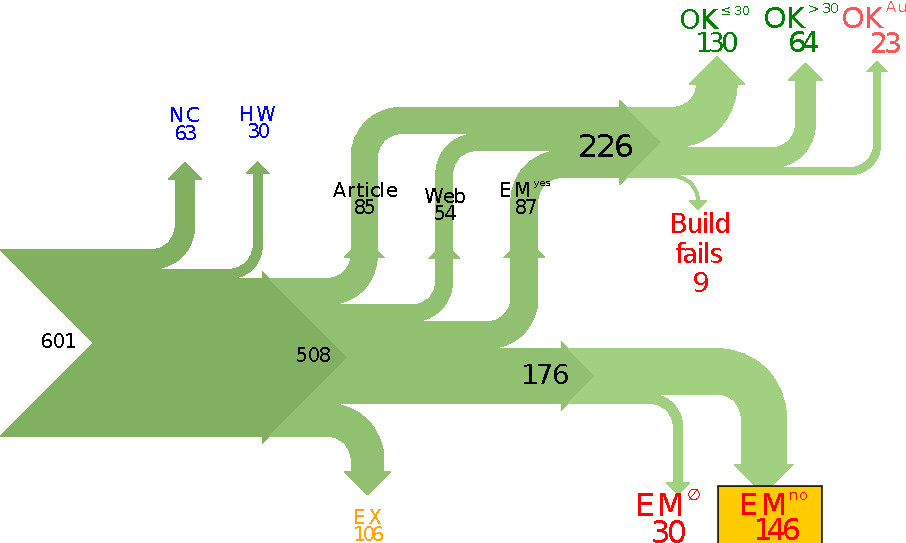
\includegraphics[height=4cm]{img/repeatability_arizona.pdf}
  \end{column}
  \begin{column}{.45\linewidth}
    \small
    \begin{itemize}
    \item 8 ACM conferences ({\scriptsize ASPLOS'12, CCS'12, OOPSLA'12, OSDI'12,
      PLDI'12, SIGMOD'12, SOSP'11, VLDB'12}) and 5 journals
    \item 
      $\text{EM}^{\text{no}}$= \alert{the code cannot be provided}
    \end{itemize}
  \end{column}
\end{columns}
\end{frame}

\begin{frame}[label=sec-1-0-4]{The Dog Ate my Homework !!! }
  \vspace{-.4cm}
  \begin{multicols}{2}
    \begin{itemize}[<+->]
    \item \alert<.>{Versioning Problems}
    \item \alert<.>{Bad Backup Practices}
    \item \alert<.>{Code Will be Available Soon}
    \item \alert<.>{No Intention to Release}
    \item \alert<.>{Programmer Left}
    \item \alert<.>{Commercial Code}
    \item \alert<.>{Proprietary Academic Code}
    \item \alert<.>{Research vs. Sharing}
    \item<.-> ...
    \item<.-> ...
    \end{itemize}
  \end{multicols}
%  \vspace{-.5cm}

  \begin{block}{}
  \vspace{-.4cm}
  \begin{overlayarea}{\linewidth}{5cm}
      \small
      \only<1>{
        \begin{quote}
          Thanks for your interest in the implementation of our
          paper. The good news is that I was able to find some code. I
          am just \alert{hoping} that \alert{it} is a stable working
          version of the code, and \alert{matches the implementation we
            finally used for the paper}. Unfortunately, I have
          \alert{lost some data} when \alert{my laptop was stolen} last
          year. The bad news is that the code is not commented and/or
          clean.
        \end{quote}
        \begin{quote}
          Attached is the $\langle$system$\rangle$ source code of our
          algorithm. I’m \alert{not} very \alert{sure whether it is the
            final version of the code used in our paper}, but it should
          be at least 99\% close. Hope it will help.
        \end{quote}}%
      \only<2>{
        \begin{quote}
          Unfortunately, the server in which my implementation was
          stored had a \alert{disk crash in April and three disks
            crashed simultaneously}. While the help desk made
          significant effort to save the data, my entire implementation
          for this paper was not found.
        \end{quote}}
      \only<3>{
        \begin{quote}
          Unfortunately the
          current system is \alert{not mature enough at the moment}, so
          it’s not yet publicly available. We are actively working on a
          number of extensions and \alert{things are somewhat
            volatile}. However, once things stabilize we plan to release
          it to outside users. At that point, we would be happy to send
          you a copy.
        \end{quote}}%
      \only<4>{
        \begin{quote}
          I am afraid that the source code was never released. The code
          was \alert{never intended to be released so is not in any shape
            for general use}.
        \end{quote}}%
      \only<5>{
        \begin{quote}
          $\langle$STUDENT$\rangle$ was a graduate student in our
          program but \alert{he left a while back} so I am responding
          instead. For the paper we used a prototype that included many
          moving pieces that only $\langle$STUDENT$\rangle$ knew how to
          operate and we did not have the time to integrate them in a
          ready-to-share implementation before he left. Still, I hope
          you can build on the ideas/technique of the paper. 
        \end{quote}
        \begin{quote}
          Unfortunately, the author who has done most of the coding for
          this paper has \alert{passed away} and the code is no longer
          maintained.
        \end{quote}
      }%
      \only<6>{
        \begin{quote}
          Since this work has been done at $\langle$COMPANY$\rangle$
          \alert{we don't open-source code} unless there is a compelling
          business reason to do so. So unfortunately I don’t think we’ll
          be able to share it with you.
        \end{quote}
        \begin{quote}
          The code \alert{owned by $\langle$COMPANY$\rangle$}, and AFAIK
          the code is not open-source.  Your best bet is to reimplement
          :( Sorry.
        \end{quote}}%
      \only<7>{
        \begin{quote}
          Unfortunately, the $\langle$SYSTEM$\rangle$
          sources are \alert{not meant to be opensource} (the code is partially
          \alert{property of $\langle$UNIVERSITY 1$\rangle$,
            $\langle$UNIVERSITY 2$\rangle$ and $\langle$UNIVERSITY
            3$\rangle$.})

          If this will change I will let you know, albeit I do not
          think there is an intention to make the
          $\langle$SYSTEM$\rangle$ sources opensource in the near
          future.
        \end{quote}
        \begin{quote}
          If you're interested in obtaining the code, \alert{we only ask
            for a description of the research project} that the code
          will be used in (\alert{which may lead to some joint
            research}), and we also have a software license agreement
          that the University would need to sign.
        \end{quote}}
      \only<8>{
        \begin{quote}
          In the past when we attempted to share it, we found ourselves
          spending more time getting outsiders up to speed than on our
          own research. So \alert{I finally had to establish the policy
            that we will not provide the source code outside the group}.
        \end{quote}
      }
    \end{overlayarea}
  \end{block}
  \null\vspace{-.4cm}
\end{frame}
 %%%%%%%%%%%%%%%%%%%%%%%%%%%%%%%%%%%%%%%%%%%%%%%%%%%%%%
\section[{\scshape Reporting}]{{\scshape Reporting} \href{https://github.com/alegrand/SMPE}{Thanks to GitHub SMPE} }
 
\label{sec-3}
\subsection{An IMRAD Report }
\label{sec-3-1}
\begin{frame}[label=sec-3-1-1]{Structure}
Research articles are often structured in this basic order:
\begin{description}
\item[{Introduction}] Why was the study undertaken? What was the research
question, the tested hypothesis or the purpose of
the research?
\item[{Methods}] When, where, and how was the study done? What
materials/hardware were used? How was it configured?
\item[{Results}] What answer was found to the research question; what did
the study find? Was the tested hypothesis true? \alert{Present
useful results in a synthetic way with a logical order}.
\item[{Discussion}] What might the answer imply and why does it matter?
How does it fit in with what other researchers have
found? What are the possible bias and points to
improve? What are the perspectives for future
research?
\end{description}

Such structure \alert{facilitates literature review} and is a very effective
way to convey information.

If the report is a few pages long then \alert{an abstract is required}.
\end{frame}
\subsection{Good Practice for Setting up a Laboratory Notebook}
\label{sec-3-2}
\begin{frame}[label=sec-3-2-1]{Step 0: Taking Notes}
\alert{Document} your:
\begin{itemize}
\item \alert{Hypotheses}: keep track of your ideas/line of thoughts
\item \alert{Experiments}: details on how and why an experiment was run, including
failed or ambiguous attempts.
\item \alert{Initial analysis or interpretation} of these experiments: was the
outcome conform to the expectation or not? does it (in)validate the
hypothesis?
\item \alert{Organization}: keep track of things to do/fix/test/improve
\end{itemize}

\alert{Structure}:
\begin{enumerate}
\item General information about the document and organization \alert{conventions}
(e.g., directory structure, notebook structure, experimental result
storing mechanism, \ldots{})
\item Documentation of \alert{commonly used commands} and of how to set up
experiments (e.g., git cloning, environment deployment, connection
to machines, compiling scripts)
\item Experiment results can be either structured \alert{by dates} ($\leadsto$ add
tags) or \alert{by experiment campaigns} ($\leadsto$ add date/time)
\end{enumerate}
\end{frame}
\begin{frame}[label=sec-3-2-2]{Which format should I use ?}
\begin{itemize}
\item \alert{Wikis} are encouraged to favor collaboration but I do not find them
really effective
\item \alert{Blogging} systems are also a way of managing such notebook but they
should rather be considered as an effective way to share information
with others
\item I recommend to use basic \alert{plain-text} format and to \alert{structure it
hierarchically}
\begin{center}
Here is a \alert{\href{http://starpu-simgrid.gforge.inria.fr/misc/LabBook.html\#sec-8-1}{link}} to an excerpt of the journal of one of my PhD
student, managed with git/org-mode. More detailed links are given in
slide~\ref{orglabref}.
\end{center}
\end{itemize}

Last but not least:
\begin{center}
Provide links to \alert{Raw Data}!!!
\end{center}
\end{frame}
\begin{frame}[label=sec-3-2-3]{When/How Often Should I Use it?}
I have a very intense usage (demo to \alert{\href{file:///Users/jvincent/org/journal.org}{general journal}} and specific
\alert{\href{file:///Users/jvincent/Work/Documents/Articles/2013/2013_boinc_response_time_optimization/journal.org}{BOINC journal}}) and I tend to capture a lot of information but you do
not have to be as extreme as I am. Here are a few advices:

\begin{itemize}
\item Spending \alert{more than an hour without} at least \alert{writing} what you're
working on \alert{is not right}\ldots{}
\begin{itemize}
\item \alert{Take a 5 minutes} break and ask yourself what you're doing, what is
keeping you busy and where all this is leading you
\end{itemize}
\item While working on something, you will often notice/think about
something you should fix/improve but you just don't want to do it
now. Take 20 seconds to write a \alert{TODO} entry.
\item There are moments where you have to \alert{wait for something} (compiling,
deployment, \ldots{}). It is generally the perfect time for improving
your notes (e.g., detail the steps to accomplish a TODO entry).
\item \alert{By the end of the day}: daily (and weekly) \alert{review!}
\begin{itemize}
\item Update your lists, write what the next steps are
\item \alert{Summarize in a 2-4 lines} (for your advisor) what you did, what was
difficult, what you learnt.
\end{itemize}
\end{itemize}
\end{frame}
\begin{frame}[label=sec-3-2-4]{Step 1: Sharing Code and Data}
\begin{overlayarea}{\linewidth}{7.6cm}\null\vspace{-.6cm}
\begin{block}{What kinds of systems are available?}
\begin{itemize}
\item "Good" - The cloud (Dropbox, Google Drive, \alert{Figshare})
\item \alert{Better} - Version control systems (SVN, \alert{Git} and Mercurial)
\item "Best" - Version control systems on the cloud (GitHub, Bitbucket)
\end{itemize}

Depends on the level of privacy you expect but you probably already
know these tools. 
\hfill\textbf{\bf Few handle GB files}...\hfill\null
\end{block}\begin{block}{Is this enough?}
\begin{enumerate}
\item Use a workflow that \alert{documents both data and process}
\item Use the machine readable \alert{CSV format}
\item Provide \alert{raw} data and \alert{meta} data, not just statistical outputs
\item \alert{Never} do data manipulation and statistical tests \alert{by hand}
\item \alert{Use R}, Python or another free software to read and process raw
data (\alert{ideally} to \alert{produce complete reports} with code, results
and prose)
\end{enumerate}
\end{block}

\end{overlayarea} \begin{flushright}\scriptsize Courtesy of Adam J. Richards\end{flushright}
\end{frame}
\begin{frame}[fragile,label=sec-3-2-5]{Step 2: Literate Programming}
 \small
\alert{Donald Knuth}: explanation of the program logic in a \alert{natural language}
\alert{interspersed with snippets of} macros and traditional \alert{source code}.

\begin{center}
I'm way too \texttt{3l33t} to program this way but that's \\
\alert{exactly what we need for writing a reproducible article/analysis!}
\end{center}
\vspace{-.5em}

\begin{block}{Org-mode (requires emacs)}
My favorite tool.
\begin{itemize}
\item plain text, very smooth, works both for html, pdf, \ldots{}
\item allows to combine all my favorite languages even with sessions
\end{itemize}
\end{block}
\begin{block}{Ipython notebook}
If you are a python user, go for it! Web app, easy to use/setup\ldots{}
\end{block}
\begin{block}{KnitR (a.k.a. Sweave)}
For non-emacs users and as a first step toward \emph{reproducible papers}:
\begin{itemize}
\item Click and play with a modern IDE (e.g., Rstudio)
\end{itemize}
\end{block}
\end{frame}
%%%%%%%%%%%%%%%%%%%%%%%%%%%%%%%%%%%%%%%%%%%%%%%%
\section[{\scshape R/knitr Crash Course}]{{\scshape R/knitr Crash Course} \href{https://github.com/alegrand/SMPE}{Thanks to GitHub SMPE} }
\label{sec-4}
\subsection{General Introduction}
\label{sec-4-1}
\end{document}

\begin{frame}[label=sec-4-1-1]{Why R?}
R is a great language for data analysis and statistics
\begin{itemize}
\item Open-source and multi-platform
\item Very expressive with high-level constructs
\item Excellent graphics
\item Widely used in academia and business
\item Very active community
\begin{itemize}
\item Documentation, FAQ on \url{http://stackoverflow.com/questions/tagged/r}
\end{itemize}
\item Great integration with other tools
\end{itemize}
\end{frame}
\begin{frame}[label=sec-4-1-2]{Why is such R a pain for computer scientists?}
\begin{itemize}
\item R is \alert{not} really a \alert{programming} language
\item Documentation is for statisticians
\item Default plots are \textit{cumbersome} (meaningful)
\item Summaries are \textit{cryptic} (precise)
\item \alert{Steep learning curve} even for us, computer scientists whereas we
generally switch seamlessly from a language to another!  That's
frustrating! ;)
\end{itemize}
\end{frame}
\begin{frame}[label=sec-4-1-3]{Do's and dont's}
\textit{R is high level, I'll do everything myself}
\begin{itemize}
\item CTAN comprises 4,334 \TeX{}, \LaTeX{}, and related packages and
tools. Most of you do not use plain \TeX{}.
\item Currently, the CRAN package repository features 4,030 available
packages.
\item How do you know which one to use??? Many of them are highly
exotic (not to say useless to you).
\begin{center}
I learnt with \url{http://www.r-bloggers.com/}
\end{center}
\end{itemize}


\begin{itemize}
\item Lots of introductions but not necessarily what you're looking
for so \alert{I'll give you a short tour}. 

You should quickly realize though that you need proper training
in statistics and data analysis if you do not want tell
nonsense.

\item Again, you should read \alert{Jain's book on The Art of Computer Systems
Performance Analysis}

\item You may want to \alert{follow online courses}:
\begin{itemize}
\item \url{https://www.coursera.org/course/compdata}
\item \url{https://www.coursera.org/course/repdata}
\end{itemize}
\end{itemize}
\end{frame}
\begin{frame}[fragile,label=sec-4-1-4]{Install and run R on debian}
 \small
\begin{verbatim}
apt-cache search r
\end{verbatim}
Err, that's not very useful :) It's the same when searching on
google but once the filter bubble is set up, it gets better\ldots{}
\begin{verbatim}
sudo apt-get install r-base
\end{verbatim}

\begin{verbatim}
R
\end{verbatim}

\scriptsize
\begin{verbatim}
R version 3.2.0 (2015-04-16) -- "Full of Ingredients"
Copyright (C) 2015 The R Foundation for Statistical Computing
Platform: x86_64-pc-linux-gnu (64-bit)

R is free software and comes with ABSOLUTELY NO WARRANTY.
You are welcome to redistribute it under certain conditions.
Type 'license()' or 'licence()' for distribution details.

R is a collaborative project with many contributors.
Type 'contributors()' for more information and
'citation()' on how to cite R or R packages in publications.

Type 'demo()' for some demos, 'help()' for on-line help, or
'help.start()' for an HTML browser interface to help.
Type 'q()' to quit R.

>
\end{verbatim}
\end{frame}

\begin{frame}[fragile,label=sec-4-1-5]{Install a few cool packages}
 R has it's own package management mechanism so just run R and type the
following commands:
\begin{itemize}
\item \texttt{ddply}, \texttt{reshape} and \texttt{ggplot2} by Hadley Wickham (\url{http://had.co.nz/})
\begin{verbatim}
install.packages("plyr")    
  # or better: install.packages("dplyr")
install.packages("reshape") 
  # or better; install.packages("tidyr")
install.packages("ggplot2")
\end{verbatim}
\item \texttt{knitR} by (Yihui Xie) \url{http://yihui.name/knitr/}
\begin{verbatim}
install.packages("knitr")
\end{verbatim}
\end{itemize}
\end{frame}
\begin{frame}[fragile,label=sec-4-1-6]{IDE}
 Using R interactively is nice but quickly becomes painful so at some
point, you'll want an IDE.

\medskip

Emacs is great but you'll need \emph{Emacs Speaks Statistics}
\begin{verbatim}
sudo apt-get install ess
\end{verbatim}
\medskip

\begin{center}
In this tutorial, I will briefly show you \alert{rstudio}
(\url{https://www.rstudio.com/}) and later how to use \texttt{org-mode}
\end{center}
\end{frame}
\subsection{Reproducible Documents: knitR}
\label{sec-4-2}
\begin{frame}[label=sec-4-2-1]{Rstudio screenshot}
\vspace{-.5cm}
\begin{center}
  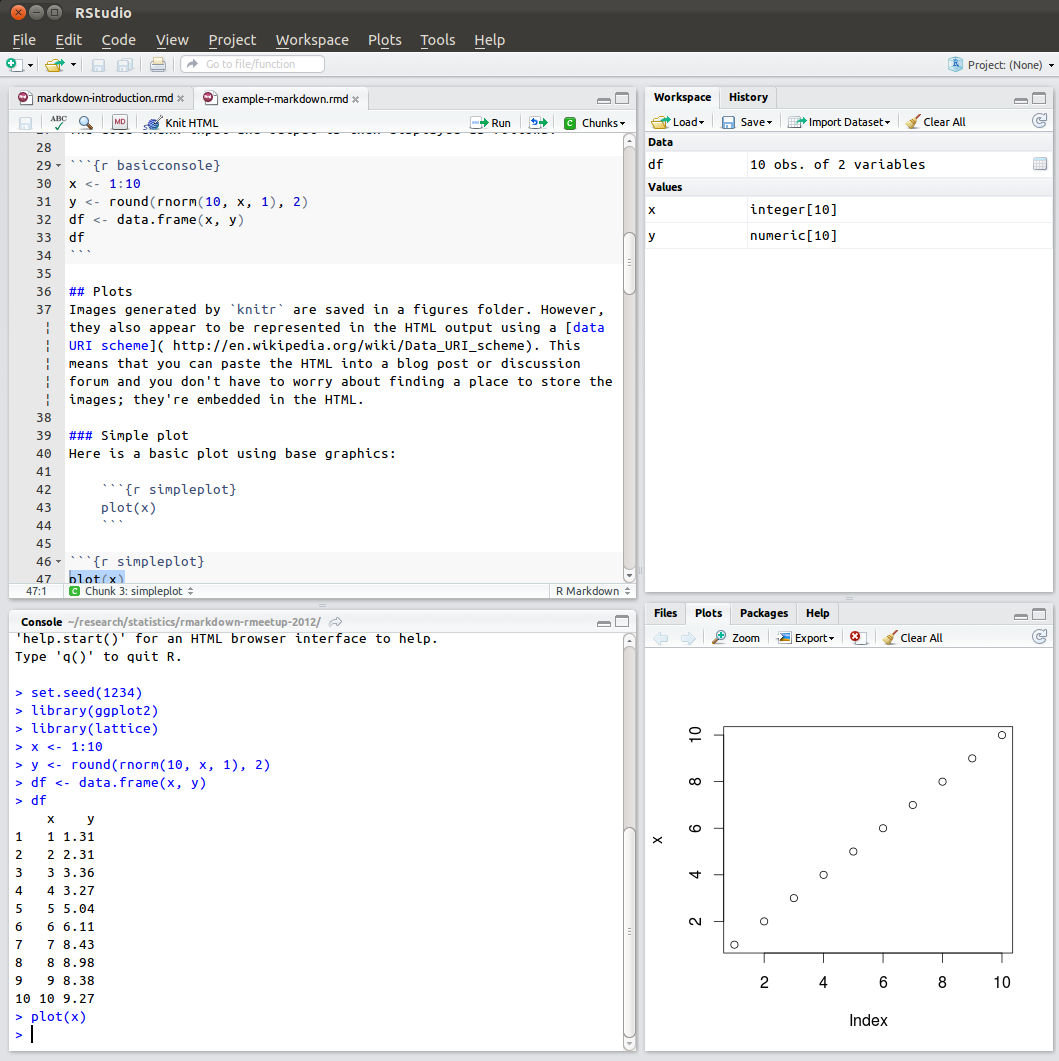
\includegraphics[height=9cm]{./img/rstudio_shot.png}
\end{center}
\end{frame}
\begin{frame}[fragile,label=sec-4-2-2]{Reproducible analysis in Markdown + R}
 \begin{itemize}
\item Create a new \alert{R Markdown} document (Rmd) in rstudio
\item R chunks are interspersed with \texttt{```\{r\}} and \texttt{```}
\item Inline R code: \texttt{`r sin(2+2)`}
\item You can \alert{knit} the document and share it via \alert{rpubs}
\item R chunks can be sent to the top-level with \texttt{Alt-Ctrl-c}
\item I usually work mostly with the current environment and only knit in
the end
\item Other engines can be used (use rstudio \alert{completion})
\begin{verbatim}
```{r engine='sh'}
ls /tmp/
```
\end{verbatim}
\item Makes \alert{reproducible analysis as simple as one click}
\item Great tool for quick analysis for self and colleagues, homeworks, \ldots{}
\end{itemize}
\end{frame}
\begin{frame}[fragile,label=sec-4-2-3]{Reproducible articles with \LaTeX{} + R}
 \begin{itemize}
\item Create a new \alert{R Sweave} document (Rnw) in rstudio
\item R chunks are interspersed with 
\texttt{<\null<>\null>=}
and \texttt{@}
\item You can \alert{knit} the document to produce a pdf
\item You'll probably quickly want to \alert{change default behavior} (activate
the cache, hide code, \ldots{}). In the preembule:
\begin{verbatim}
<<echo=FALSE>>=
opts_chunk$set(cache=TRUE,dpi=300,echo=FALSE,fig.width=7,
                warning=FALSE,message=FALSE)
@
\end{verbatim}
\item Great for journal articles, theses, books, \ldots{}
\end{itemize}
\end{frame}


%%%%%%%%%%%%%%%%%%%%%%%%%%%%%%%%%%%%%%%%%%%%%%%%%%%%%%
%%%%%%%%%%%%%%%%%%%%%%%%%%%%%%%%%%%%%%%%%%%%%%%%%%%%%%
\end{document}
